\documentclass{article}
\usepackage{graphicx} % Required for inserting images
\usepackage{geometry} 

\title{Práctica 1: Procesado Digital de Imágenes usando Python}
\author{Mario García Berenguer, Adonis García Anés}
\date{October 2024}

\begin{document}

\maketitle
Práctica para la Asignatura de Arquitecturas y Algortimos para el Procesamiento de Imágenes
\centering
\includegraphics[width=0.15\textwidth]{logoUPM.png}

\section{Introducción}
\raggedright
Para esta práctica se nos ha facilitado una imagen con la que trabajar, a la cual la debíamos de realizar una serie de transformaciones tanto en el dominio de la imagen como en el dominio de su frecuencia. La imagen facilitada es la siguiente:
\\
\vspace{0.5cm}
\centering
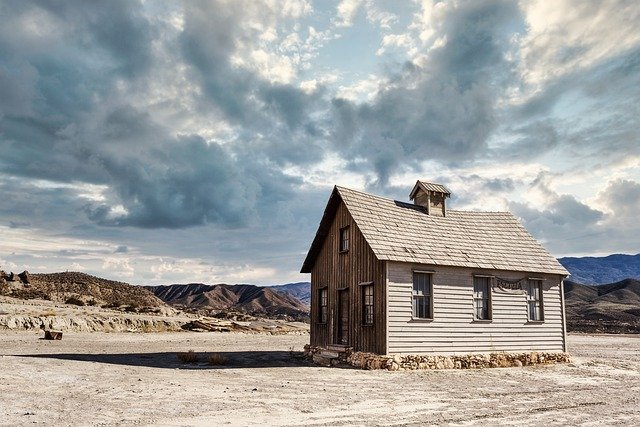
\includegraphics[width=0.5\textwidth]{Landscape.jpg}
\raggedright
\\
Todas las Tareas se han realizado a través de un Jupyter Notebook en Python.
\section{Tarea: Visualización de la Imagen}

En este primer apartado debemos visualizar tanto la imagen original como cada uno de sus tres canales de color por separado.

\centering
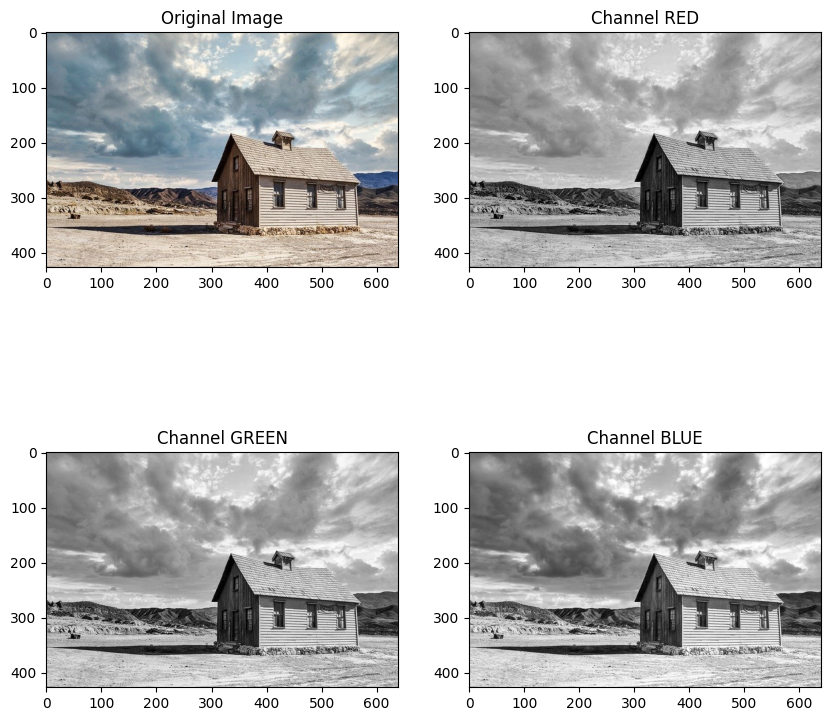
\includegraphics[width=15cm]{Tarea1.png}
\raggedright

Como podemos ver, no parece que ningún canal sobresalga sobre el resto, y los tres canales RGBs parecen bastante nivelados.

\section{Tarea: Cálculo de Valores estadísticos}

A continuación vamos a estudiar la distribución de los valores de cada uno de los colores, calculando la media y la desviación típica de los mismos para comprobar si es cierto que los 3 canales están nivelados. En la tabla a continuación se muestran los resultados.
\[
\begin{tabular}{|c|c|c|c|}
    \hline
    Canales & Media & Desviación Típica \\ \hline
    Canal Rojo & $157.821838$ & $52.427288$ \\ \hline
    Canal Azul & $157.323233$ & $56.728633$ \\ \hline
    Canal Verde & $159.220506$ & $53.888831$ \\ \hline
\end{tabular}
\]
Podemos observar que, aunque la diferencia entre los tres canales es muy poco significativa, el canal con mayor valor medio es el Verde y el canal con mayor desviación típica es el Azul, seguramente por su alta presencia en el cielo pero su escasa presencia en la tierra o la casa.

\section{Tarea: Operaciones Aritméticas y Booleanas}

Para esta tarea se nos proponía realizar sobre los canales con mayor y menor varianza (en nuestro caso el azul y el rojo) una serie de operaciones tanto aritméticas como booleanas, véase suma, resta, OR y AND. Estas últimas deben realizarse con las imágenes binarizadas, por lo que tuvimos que asignar a todos los valores de la imagen valor 0 o 255. Esto se hizo con una simple aproximación. A continuación el resultado.

\centering
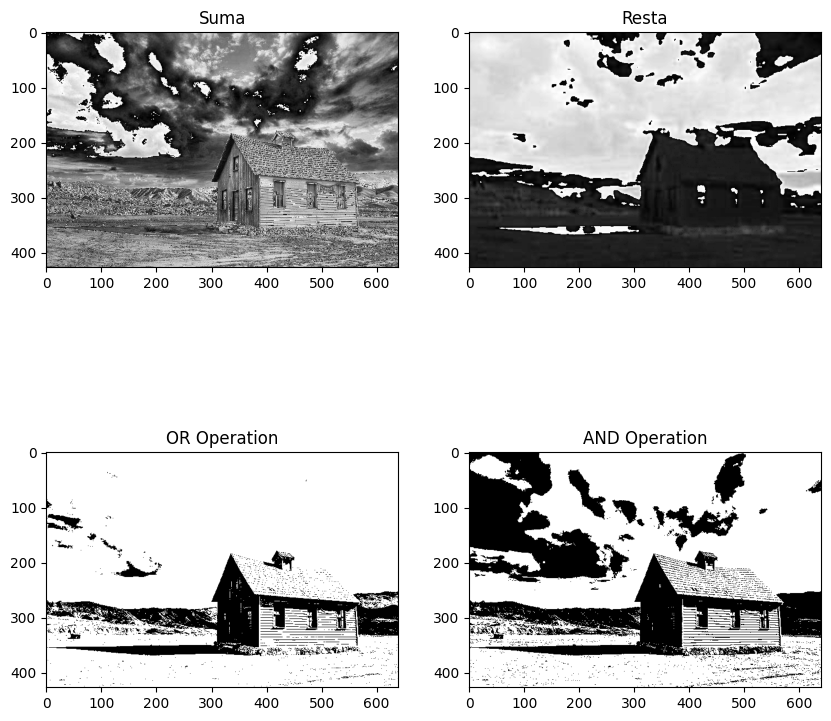
\includegraphics[width=15cm]{Tarea3.png}
\raggedright

La suma de colores da un resultado bastante similar al original, mientras que la resta no nos permite apenas distinguir la casa o el fondo. Las operaciones booleanas son un tanto diferentes, ya que en el caso del OR se encuentran en blanco las zonas donde el valor rojo o azul superaba los 127, mientras que en el AND ambos valores deben superar ese umbral para que aparezca el color blanco, de ahí que se aprecien más zonas negras.

\section{Tarea: Cálculo de Histograma}

En este apartado debíamos calcular el histograma de grises para cada uno de los canales de color, a la vez que lo haciamos para cada imagen generada con las operaciones de la Tarea 3. 

\centering
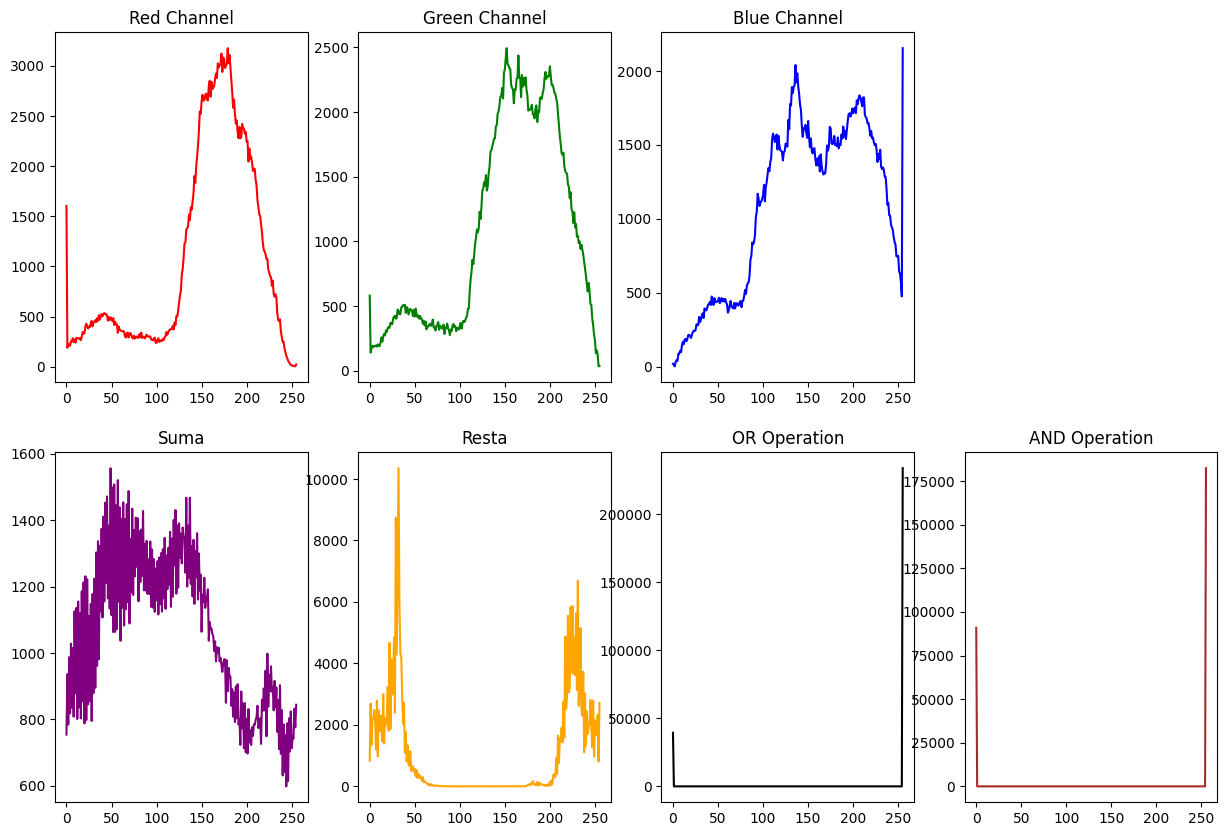
\includegraphics[width=15cm]{Tarea4.png}
\raggedright

Se observa que, como es de esperar, los histogramas de las operaciones OR y AND solo presentan el valor 0 y el valor 255. Además, en la resta se puede ver que los valores intermedios, que son los predominantes, han desaparecido practicamente.

\section{Tarea: Filtrado en el Dominio Espacial}

A continuación se implementan una serie de filtros tanto de paso bajo como de realzado de bordes. Se utilizan kernels $3x3$ y $5x5$ para esta tarea. Los filtros de paso bajo van a realizar un suavizado de la imagen ponderando todos los valores y creando áreas más homogéneas. Por el contrario, los filtros de paso alto van a realzar los bordes y a disminuir el número de áreas homogéneas. Todo esto se puede apreciar en la siguiente figura.

\centering
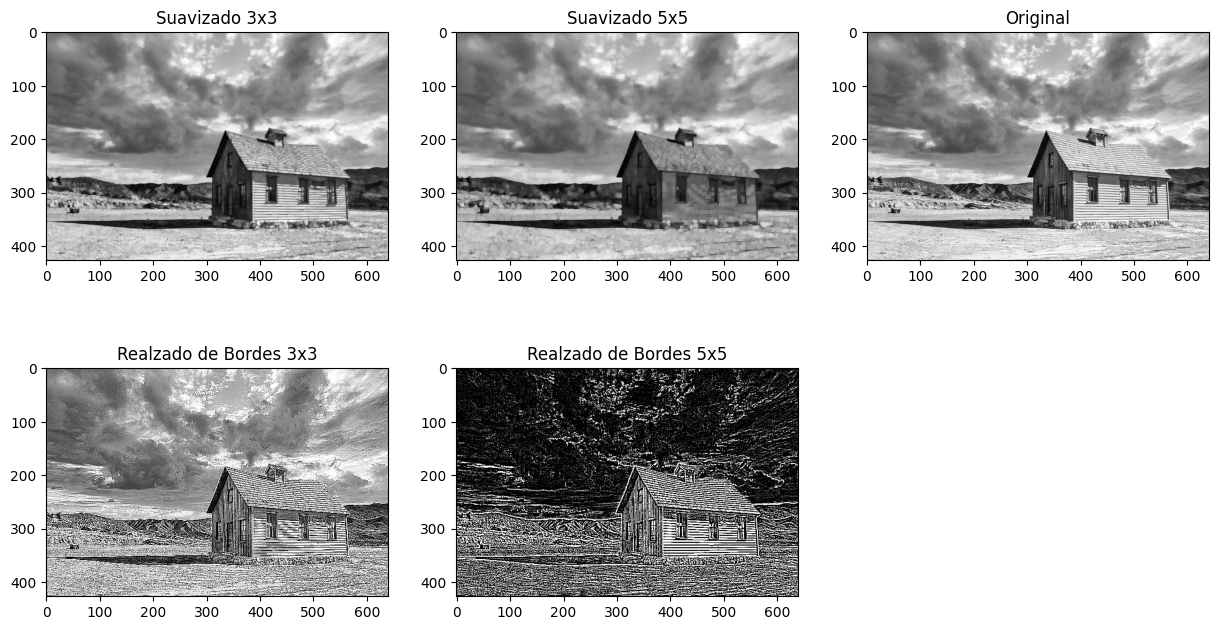
\includegraphics[width=15cm]{Tarea5.png}
\raggedright

\section{Tarea: Transformada de Fourier}

El objetivo de esta tarea era visualizar la Transformada de Fourier de la Imagen con su espectro de magnitud.

\centering
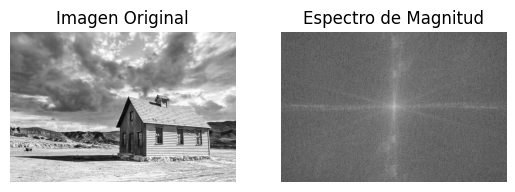
\includegraphics[width=15cm]{Tarea6.png}
\raggedright

En este espectro se puede apreciar una singularidad en el centro de la que parten 8 haces: 2 verticalmente, 2 horizontalmente y 4 en cada diagonal.

\section{Tarea: Filtrado en el dominio de Fourier}

Como se ha demostrado teóricamente, un filtro convolucional en el dominio espacial de la imagen equivale a multiplicar su transformada de Fourier por una máscara en el dominio de la frecuencia. Es por esto que somos capaces de dada la transformada, crear diversos filtros con forma circular tanto de paso bajo como de paso alto, y gracias a la transformada inversa conseguir la de nuevo la imagen filtrada. 

A continuación se presentan tres máscaras para realizar filtros de paso bajo. Estas tiene forma circular y son de radio $10$, $20$, y $30$ respectivamente.

\centering
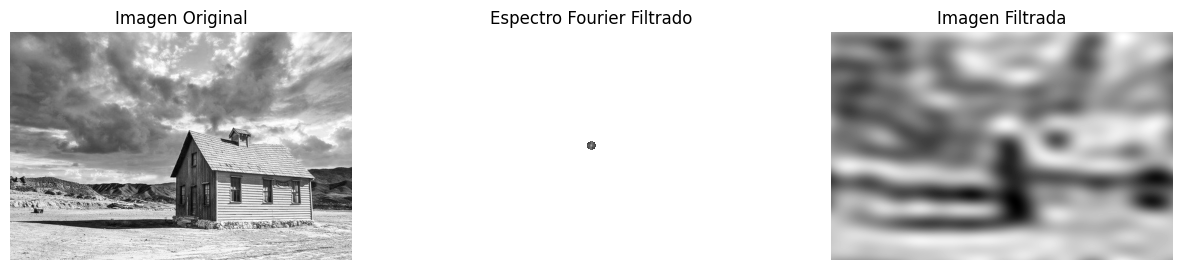
\includegraphics[width=15cm]{Tarea7_suav10.png}
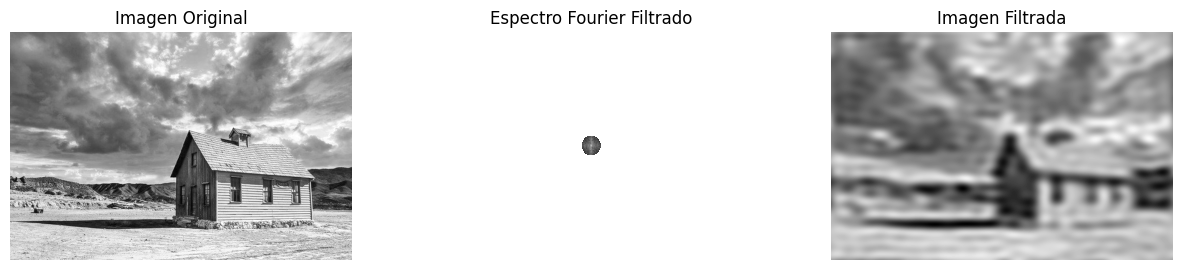
\includegraphics[width=15cm]{Tarea7_suav20.png}
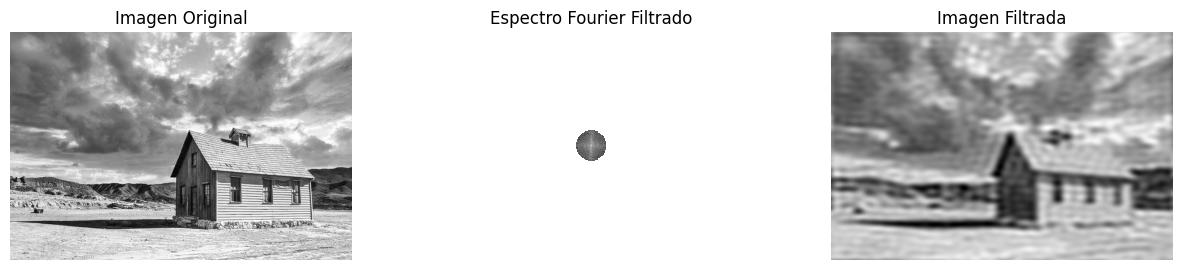
\includegraphics[width=15cm]{Tarea7_suav30.png}
\raggedright

Vemos un claro efecto de suavizado cuanto menos es el radio del círculo, ya que este obtendrá frecuencias cada vez más homogéneas.
\\
Si nos vamos al caso opuesto, los filtros de paso alto, están construidos de la misma manera pero generan el efecto opuesto.

\centering
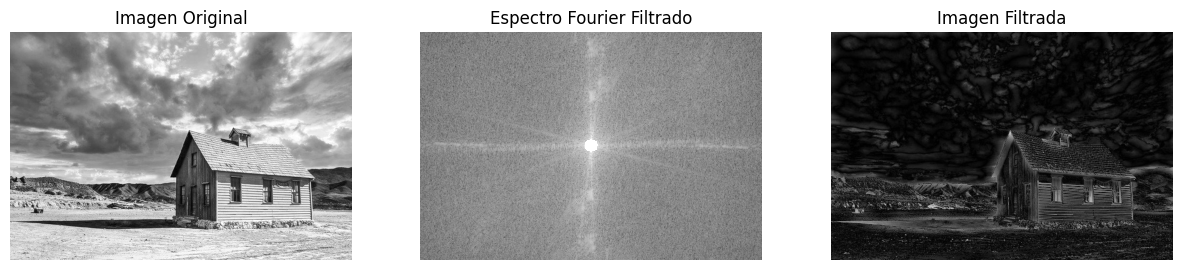
\includegraphics[width=15cm]{Tarea7_bordes10.png}
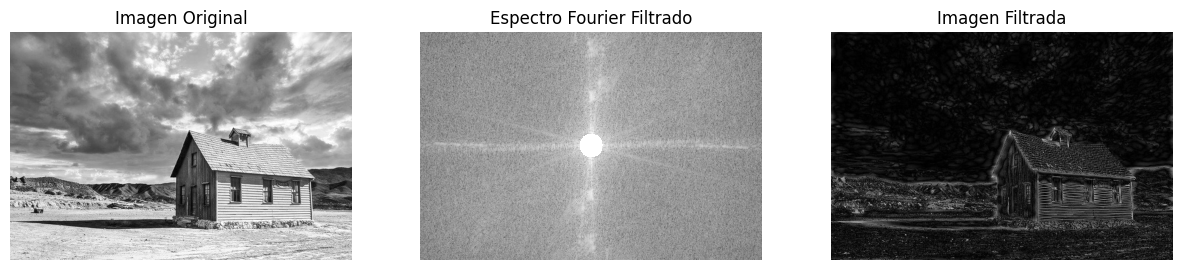
\includegraphics[width=15cm]{Tarea7_bordes20.png}
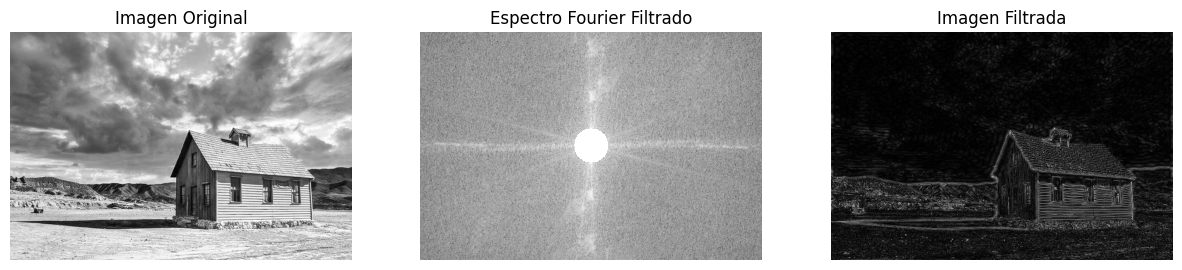
\includegraphics[width=15cm]{Tarea7_bordes30.png}
\raggedright

En este caso nos quedamos con toda la transformada menos con la parte central, lo que provoca que eliminemos las partes más homogéneas y como resultado obtengamos un realce de los bordes. En este caso cuanto más grande es el radio más se realzan, ya que eliminas mayor cantidad de homogeneidad de la imagen.

\end{document}
